\documentclass[12pt]{article}
\usepackage{amsmath}
\usepackage{amsfonts}
\usepackage{amssymb}
\usepackage{graphicx}
\usepackage{geometry}
\usepackage{tocloft}
\geometry{a4paper, margin=1in}
\linespread{2.0}
\begin{document}

\begin{titlepage}
    \centering
    
    {\Huge\bfseries Application and Optimization of Path Planning Algorithms\par}
    
    \vspace{1in}
    
    {\Large\itshape How can mathematical optimization enhance the performance of A* and RRT* path planning algorithms in dynamic environments?\par}
    
    \vspace{1in}
    
    {\Large Mathematics Analysis \& Approaches HL\par}

    \vspace{1in}
    
    {\Large Word Count: 2481\par} % Replace XXXX with the actual word count

\end{titlepage}
\tableofcontents

\newpage
\section{Introduction}
Path Planning, a critical branch of robotics and machine learning, refers to developing a route from a start point to a destination that an object must follow to avoid obstacles. However, we cannot just accept any path, so the optimization of distance, time, safety, and other criteria is always necessary. 
From ancient maps to modern autonomous GPS navigation, the challenge of effective navigation in dynamic environments remains crucial. Dynamic Environments are characterized by their unpredictable nature, which may include moving obstacles, alternating terrain, and various conditions, that require algorithms to adapt and respond in real-time. Traditional path-planning algorithms have demonstrated their usage in static environments, but struggle in dynamic environments. 
The pursuit of a “complete” algorithm for such environments involves not only navigating efficiently and safely but also being able to adapt continually along the way. The aim of this essay, therefore, is to firstly comprehend the mathematical background of path-planning algorithms. After that, conducting a case study will be necessary for two situations, where one is that the environment is familiar, and the other one is that the environment is unfamiliar. This is followed by the evaluation of the A* and RRT* algorithms, which are both known for their decent optimality and will then further be optimized using various advanced techniques. This leads to my research question: \textbf{“To what extent can I find the most complete path-planning algorithm in dynamic Environments?”}

\newpage
\section{Notations Used}
\begin{center}
\begin{tabular}{ll}
$\Rightarrow$ $\mathbf{G = (V, E)}$ & \begin{minipage}[t]{0.75\textwidth}
\textbf{G}: It’s the graph itself, a structure to model pairwise relations.\\
\textbf{V}: Represents the set of vertices (nodes) in the graph.\\
\textbf{E}: Represents the set of edges (connections) in the graph.
\end{minipage} \\[1em]

$\Rightarrow$ $\mathbf{w(u, v)}$ & \begin{minipage}[t]{0.75\textwidth}
\textbf{w}: The cost of moving from the edge of node $u$ to node $v$.\\
\textbf{u}: Node $u$ is the initial node.\\
\textbf{v}: Node $v$ is the final node.
\end{minipage} \\[1em]

$\Rightarrow$ $\mathbf{S}$ & \begin{minipage}[t]{0.75\textwidth}
\textbf{S}: The start node, it’s where the path begins.
\end{minipage} \\[1em]

$\Rightarrow$ $\mathbf{T}$ & \begin{minipage}[t]{0.75\textwidth}
\textbf{T}: The target node, it’s where the path ends.
\end{minipage} \\[1em]

$\Rightarrow$ $\mathbf{d(u, v)}$ & \begin{minipage}[t]{0.75\textwidth}
\textbf{d}: The direct cost of moving from node $u$ to node $v$.\\
\textbf{u}: Node $u$ is the initial node.\\
\textbf{v}: Node $v$ is the final node.
\end{minipage} \\[1em]

$\Rightarrow$ $\mathbf{f(n) = g(n) + h(n)}$ & \begin{minipage}[t]{0.75\textwidth}
\textbf{f(n)}: The total cost function in A*.\\
\textbf{g(n)}: The actual cost from $S$ to a certain node $n$.\\
\textbf{h(n)}: The estimated cost from node $n$ to $T$.
\end{minipage} \\[1em]

$\Rightarrow$ $\mathbf{N}$ & \begin{minipage}[t]{0.75\textwidth}
\textbf{N}: A set that includes all adjacent nodes of a single node.
\end{minipage} \\[1em]

$\Rightarrow$ $\mathbf{P}$ & \begin{minipage}[t]{0.75\textwidth}
\textbf{P}: The path of nodes from $S$ to $T$.
\end{minipage} \\[1em]

$\Rightarrow$ $\mathbf{O}$ and $\mathbf{C}$ & \begin{minipage}[t]{0.75\textwidth}
\textbf{O}: Open set of nodes that need to be explored.\\
\textbf{C}: Closed set of nodes that have been fully explored.
\end{minipage} \\[1em]

\end{tabular}
\end{center}
\newpage
\section{Introduction to Path Planning Algorithms}
Path planning algorithms can be classified into two categories, namely global and local path planning algorithms. Global path planning algorithms are designed to compute a path from start to finish by considering the whole environment. These algorithms aim to find the optimal path based on distance, safety or visibility in most cases. 				One example that I will delve deeper into is the RRT* algorithm, whilst measuring its path cost, path length, time required to generate the path and memory usage. On the other hand, local path planning algorithms are not aware of the whole environment. They make decisions based on local information available at the medium's current location. They are often used in dynamic environments and can further be classified into evolutionary and heuristic path planning algorithms; however, evolutionary algorithms are based on biological concepts rather than mathematical. Thus, I will delve deeper into a heuristic algorithm, namely the A* algorithm and measure the same performance metrics as the RRT* algorithm, in order to determine the more complete algorithm before and after the utilisation of various optimization techniques. 
\begin{figure}[h!]

  \centering
  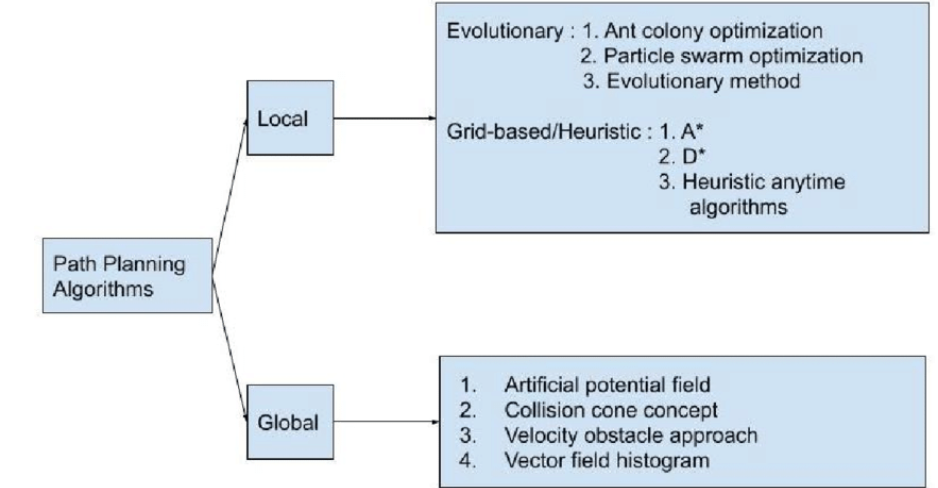
\includegraphics[width=0.5\textwidth]{Screenshot 2024-06-05 083017.png}
    \caption{Classification of Path Planning Algorithms}
\end{figure}
\newpage
\subsection{Performance Metrics}
The first important performance metric, as previously mentioned, is the path length which measures the total length, or cost, of the path found by the algorithm. This metric is crucial for evaluating the completeness of a path in terms of travel distance, or cost, which        implies the resource usage for example fuel or time. 
Secondly, time complexity is referred to the total time taken from the start of the algorithm until a path is found. This is a very important measure for applications where decision time is limited, such as real-time systems and especially in dynamic environments where change can occur unpredictable. 
Another important performance metric is the memory usage, which is the amount of memory required during the execution of the algorithm and directly correlates with the size of the data structures used. It is essential for evaluating the performance of algorithms in environments with limited computational resources. 
Lastly, it is also important to recognize the general trend of scalability. This defines how well the algorithm performs as the size of the environment increases and is important for determining the algorithm’s applicability to large-scale problems. 
\begin{figure}[h!]

  \centering
  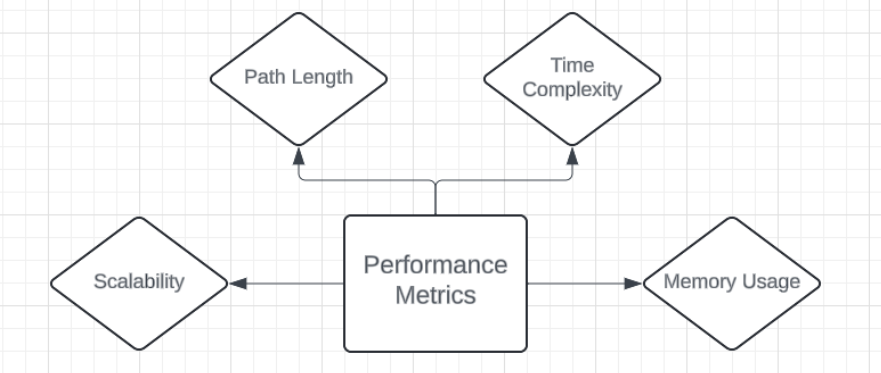
\includegraphics[width=0.5\textwidth]{Screenshot 2024-06-05 084029.png}
    \caption{Performance Metrics Flowchart}
\end{figure}
\newpage
\subsection{The Euler-Lagrange Equation}
The Euler-Lagrange equation is a differential equation whose solutions are the functions that make a functional reach its extremum (maximum or minimum). In the context of path planning, the functional typically represents the cost associated with a path.

Given a functional \( J[y] \) defined as:

\[
J[y] = \int_{a}^{b} L(x, y, y') \, dx
\]

where \( L \) is the Lagrangian, which depends on \( x \), the function \( y(x) \), and its derivative \( y'(x) \), the Euler-Lagrange equation is:

\[
\frac{\partial L}{\partial y} - \frac{d}{dx} \left( \frac{\partial L}{\partial y'} \right) = 0
\]

In path planning, the functional \( J[y] \) often represents the total cost, such as the total distance traveled or the energy expended. By finding the function \( y(x) \) that minimizes (or maximizes) this functional, we can determine the optimal path.

For example, consider a functional representing the total distance:

\[
J[y] = \int_{a}^{b} \sqrt{1 + \left( y'(x) \right)^2} \, dx
\]

Here, the Lagrangian is \( L(x, y, y') = \sqrt{1 + (y')^2} \). Applying the Euler-Lagrange equation:

\[
\frac{\partial L}{\partial y} - \frac{d}{dx} \left( \frac{\partial L}{\partial y'} \right) = 0
\]

Since \( L \) does not explicitly depend on \( y \), \( \frac{\partial L}{\partial y} = 0 \), and:

\[
- \frac{d}{dx} \left( \frac{y'}{\sqrt{1 + (y')^2}} \right) = 0
\]

This simplifies to:

\[
\frac{y'}{\sqrt{1 + (y')^2}} = C
\]

where \( C \) is a constant. Solving this differential equation gives the optimal path \( y(x) \).

Partial derivatives measure how a function changes as its variables change. For a function \( f(x, y) \), the partial derivative with respect to \( x \) is:

\[
\frac{\partial f}{\partial x} = \lim_{\Delta x \to 0} \frac{f(x + \Delta x, y) - f(x, y)}{\Delta x}
\]

This represents the rate of change of \( f \) with respect to \( x \), holding \( y \) constant. Partial derivatives are essential in formulating the Euler-Lagrange equation and solving optimization problems in path planning. An ordinary differential equation involves functions of one independent variable and their derivatives. The general form of an ODE is:

\[
F(x, y, y', y'', \ldots, y^{(n)}) = 0
\]

where \( y^{(n)} \) denotes the \( n \)-th derivative of \( y \) with respect to \( x \).
A classic example of an ODE is the equation for a simple harmonic oscillator:

\[
\frac{d^2 y}{dx^2} + \omega^2 y = 0
\]

The general solution to this second-order linear differential equation is:

\[
y(x) = A \cos(\omega x) + B \sin(\omega x)
\]

where \( A \) and \( B \) are constants determined by initial conditions.





\subsection{Graph Theory and Linear Algebra}
\begin{figure}[h!]

  \centering
  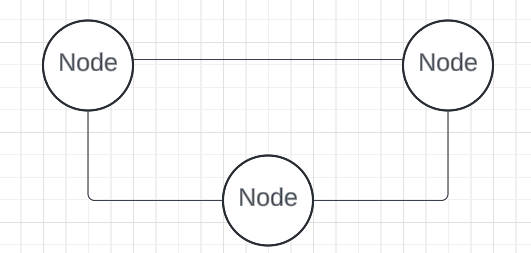
\includegraphics[width=0.5\textwidth]{Screenshot 2024-05-16 141959.png}
    \caption{\textit{Undirected Graph With Three Nodes} }
\end{figure}
In mathematics, graph theory is the study of graphs, which are mathematical structures used to model pairwise relations between objects and also how algorithms are able to iterate paths. A graph, \( G \), is an ordered pair \( G = (V, E) \), where \( V \) is a set of vertices (nodes) and \( E \subseteq \{\{x, y\} \mid x, y \in V \text{ and } x \neq y\} \), is a set of edges (links), which is an unordered pair of nodes. In simple terms, an environment of nodes, as shown in figure 3, is connected by edges and is what allows algorithms to iterate paths along. This is called an undirected simple graph.

\begin{figure}[h!]

  \centering
  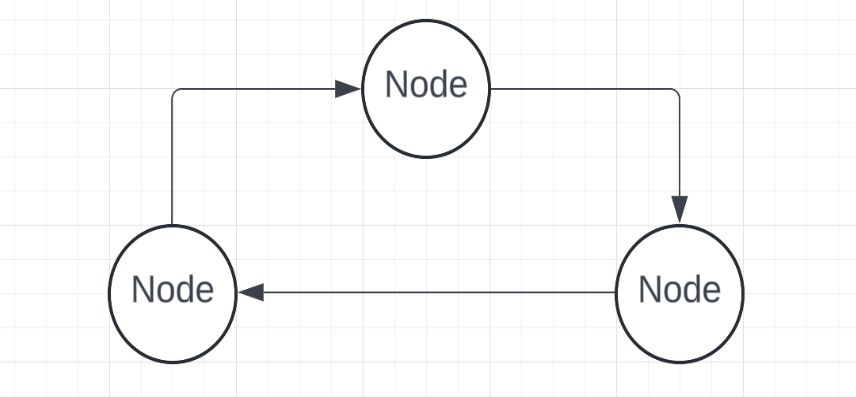
\includegraphics[width=0.5\textwidth]{Screenshot 2024-06-05 112230.png}
    \caption{\textit{Directed Graph With Three Nodes} }
\end{figure}
Similar to an undirected simple graph, the directed simple graph, \( G \), is also an ordered pair of \( G = (V, E) \), where \( V \) is a set of nodes and \( E \subseteq \{\{x, y\} \mid x, y \in V^2 \text{ and } x \neq y\} \), is a set of directed edges, which are ordered pairs of nodes. This can be seen in figure 4, where each edge has a direction that points towards a different node. One example of an undirected graph is a social network, where edges represent friendships. If person A is friends with person B, then person B is also friends with person A. On the other hand, an example of a directed graph is a social media network, where follows represent nodes. If person A follows person B, person B doesn’t necessarily follow back and might be following another person C and the amount of followings can be represented as degrees. However, each node has a certain degree, which can be split into In-Degree and Out-Degree. The amount of edges coming into a certain node is called In-Degree and the amount of edges going out of a certain node is called Out-Degree.
In graph theory, these graphs are more optimally represented as an adjacency matrix. The adjacency matrix \( A \) is an \( n \times n \) square matrix used to represent a finite graph. For an undirected graph, the adjacency matrix is symmetric, while for a directed graph, it is not necessarily symmetric.

An example of an adjacency matrix for an undirected graph with 4 nodes is:

\[
A = \begin{bmatrix}
0 & 1 & 0 & 1 \\
1 & 0 & 1 & 0 \\
0 & 1 & 0 & 1 \\
1 & 0 & 1 & 0
\end{bmatrix}
\]

In an undirected graph the adjacency matrix will always be revserings since there it does not matter as long as its nodes adjacent to edges.

An example of an adjacency matrix for a directed graph with 4 nodes is:

  - For the edge (1 → 2), set \( A[1][2] = 1 \)
   - For the edge (2 → 3), set \( A[2][3] = 1 \)
   - For the edge (3 → 1), set \( A[3][1] = 1 \)
   - For the edge (3 → 4), set \( A[3][4] = 1 \)

   The adjacency matrix \( A \) becomes:

   \[
   A = \begin{bmatrix}
   0 & 1 & 0 & 0 \\
   0 & 0 & 1 & 0 \\
   1 & 0 & 0 & 1 \\
   0 & 0 & 0 & 0
   \end{bmatrix}
   \]

This is because of following:\\
- \( A[1][2] = 1 \) indicates a directed edge from node 1 to node 2.\\
- \( A[2][3] = 1 \) indicates a directed edge from node 2 to node 3.\\
- \( A[3][1] = 1 \) indicates a directed edge from node 3 to node 1.\\
- \( A[3][4] = 1 \) indicates a directed edge from node 3 to node 4.\\
- All other entries are 0, indicating no direct edges between those nodes\\
Adjacency matrices play a crucial role in path planning algorithms. Path planning algorithms, such as Dijkstra's algorithm, A* search algorithm, and Floyd-Warshall algorithm, utilize the adjacency matrix to efficiently find the shortest path between nodes in a graph. The A* search algorithm combines the actual distance from the start node to the current node and an estimated distance from the current node to the goal node. The adjacency matrix is used to find the neighbors of the current node and to calculate the actual distance. The adjacency matrix provides a compact and efficient way to represent the connections and distances between nodes in a graph, enabling path planning algorithms to operate effectively. 


\newpage 
\section{Case Study}
\subsection{Local Path-Planning}

Local path planning is related to short-range movements and real-time adjustments based on the medium's current surroundings. This involves reacting to dynamic changes in the environment, such as moving obstacles. The scope of the local path planning is typically limited to a predefined area around the robot. This can be visualised as a moving window that shifts as the robot progresses, allowing it to focus on immediate obstacles and navigable paths.

\subsubsection{A* Algorithm}
The A* algorithm finds the shortest path from a start node to a goal node in a graph, using a heuristic to guide the search efficiently. The environment within the A* algorithm is identical to an undirected but weighted graph displayed as $G = (V, E)$. The weighted (cost) function of the A* combines two components:

\[
f(x) = g(x) + h(x)
\]

where $g(x)$ is the cost from the start node to the current node $x$ and $h(x)$ is the heuristic estimate of the cost from the current node $x$ to the goal node. The heuristic function $h(x)$ must be kept admissible, implying that it never overestimated the true cost to reach the goal.

The most used heuristic function $h(x)$ is the euclidean distance that can be displayed as:

\[
h_{2D}(x) = \sqrt{(x_{\text{goal}} - x_{\text{current}})^2 + (y_{\text{goal}} - y_{\text{current}})^2}
\]

\[
h_{3D}(x) = \sqrt{(x_{\text{goal}} - x_{\text{current}})^2 + (y_{\text{goal}} - y_{\text{current}})^2 + (z_{\text{goal}} - z_{\text{current}})^2}
\]
Another very popular heuristic function used within the A* Algorithm is the Manhattan Distance, which uses slightly less operations and therefore is more efficient; however, the Manhattan Distance is an even more inaccurate estimate of the actual shortest path. This can be represented as:
\[
h_{2D}(x) = |{x_{\text{goal}} - x_{\text{current}}| + |y_{\text{goal}} - y_{\text{current}}}|
\]

\[
h_{3D}(x) = |{x_{\text{goal}} - x_{\text{current}}| + |y_{\text{goal}} - y_{\text{current}}| + |z_{\text{goal}} - z_{\text{current}}}|
\]
In order to be able to track in the most efficient way, there is an open set that contains the most promising nodes. On the other hand, there is a closed set that ensures all computational factors are kept efficient and in place. The main problem of the conventional A* algorithm is the fact that its heuristic function requires a lot of processing time and is only an estimate of the shortest path generated. This may be optimised using calculus and linear algebra. More specifically, I will use the euler-lagrange equation in order to solve for the most optimal path generation and an overall improvement in efficiency. Furthermore, I will use linear algebra to represent the conventional heuristic functions as adjacency matrix and apply techniques of linear algebra to optimize the path generation process. 
\newpage
\subsubsection{Optimization using Euler-Lagrange Equations}
The Euler-Lagrange equation provides the necessary condition for a functional \( J \) to be at an extremum. For a functional of the form:
\begin{equation}
    J = \int_{t_0}^{t_f} L(x(t), \dot{x}(t), t) \, dt
\end{equation}
where \( L \) is the Lagrangian, \( x(t) \) is the state variable, and \( \dot{x}(t) \) is the derivative of the state variable with respect to time, the Euler-Lagrange equation is given by:
\begin{equation}
    \frac{d}{dt} \left( \frac{\partial L}{\partial \dot{x}} \right) - \frac{\partial L}{\partial x} = 0
\end{equation}



In path planning, the goal is to find the trajectory \( x(t) \) that minimizes the cost functional \( J \). Consider a 2D path planning problem where the state variables are \( x(t) \) and \( y(t) \).



Assume the Lagrangian \( L \) includes a term for kinetic energy and a potential function \( V(x, y) \) representing the cost at position \( (x, y) \):
\begin{equation}
    L(x, y, \dot{x}, \dot{y}) = \frac{1}{2} (\dot{x}^2 + \dot{y}^2) + V(x, y)
\end{equation}

The Euler-Lagrange equations for \( x \) and \( y \) are:
\begin{equation}
    \frac{d}{dt} \left( \frac{\partial L}{\partial \dot{x}} \right) - \frac{\partial L}{\partial x} = 0
\end{equation}
\begin{equation}
    \frac{d}{dt} \left( \frac{\partial L}{\partial \dot{y}} \right) - \frac{\partial L}{\partial y} = 0
\end{equation}



First, compute the partial derivatives of \( L \):
\begin{equation}
    \frac{\partial L}{\partial \dot{x}} = \dot{x}, \quad \frac{\partial L}{\partial x} = \frac{\partial V}{\partial x}
\end{equation}
\begin{equation}
    \frac{\partial L}{\partial \dot{y}} = \dot{y}, \quad \frac{\partial L}{\partial y} = \frac{\partial V}{\partial y}
\end{equation}

Substitute these into the Euler-Lagrange equations:
\begin{equation}
    \frac{d}{dt} \left( \dot{x} \right) - \frac{\partial V}{\partial x} = 0 \implies \ddot{x} = \frac{\partial V}{\partial x}
\end{equation}
\begin{equation}
    \frac{d}{dt} \left( \dot{y} \right) - \frac{\partial V}{\partial y} = 0 \implies \ddot{y} = \frac{\partial V}{\partial y}
\end{equation}



To integrate these conditions into the A* algorithm:

\begin{enumerate}
    \item \textbf{Define the Lagrangian} in terms of the state variables \( x \) and \( y \), and their velocities \( \dot{x} \) and \( \dot{y} \):
    \begin{equation}
        L(x, y, \dot{x}, \dot{y}) = \frac{1}{2} (\dot{x}^2 + \dot{y}^2) + V(x, y)
    \end{equation}
    \item \textbf{Discretize the Problem}: Convert the continuous problem into a discrete one suitable for the A* algorithm.
    \item \textbf{Use Discrete Euler-Lagrange Equations}: Implement the discrete form of the Euler-Lagrange equations in the node expansion step of A*. For each node, calculate the optimal next node based on the derived equations:
    \begin{equation}
        \frac{x_{i+1} - 2x_i + x_{i-1}}{\Delta t^2} = \frac{\partial V}{\partial x}(x_i, y_i)
    \end{equation}
    \begin{equation}
        \frac{y_{i+1} - 2y_i + y_{i-1}}{\Delta t^2} = \frac{\partial V}{\partial y}(x_i, y_i)
    \end{equation}
    \item \textbf{Update Heuristic Function}: Use the value function derived from the Euler-Lagrange equations to update the heuristic function in the A* algorithm:
    \begin{equation}
        h(x, y) = V(x, y)
    \end{equation}
\end{enumerate}



By integrating the Euler-Lagrange equations into the A* algorithm, we ensure that the paths computed are not only the shortest but also satisfy the optimality conditions derived from the calculus of variations. By implementing this we optimize the calculations within the heuristic function while it only takes on average a couple milliseconds more to process. This enhances the accuracy of the path planning process.
\newpage

\subsubsection{Optimization using Linear Algebra}


Linear algebra and adjacency matrices provide powerful tools to optimize path planning algorithms. Matrix multiplication can be used to count paths of different lengths between nodes in a graph. For example, the \( (i,j) \)-th entry of \( A^k \) (the adjacency matrix raised to the \( k \)-th power) represents the number of paths of length \( k \) from node \( i \) to node \( j \).
Eigenvalue and eigenvector analysis of the adjacency matrix provides insights into the properties of the graph. For example, the largest eigenvalue (spectral radius) can indicate the connectivity of the graph, and the corresponding eigenvector can help identify important nodes. Singular Value Decomposition can be used to approximate large adjacency matrices, reducing computational complexity. This is useful for large-scale path planning problems where directly working with the full adjacency matrix is impractical. The graph Laplacian matrix, derived from the adjacency matrix, is used in spectral clustering to partition the graph into clusters. This can simplify path planning by reducing the problem to smaller subproblems within each cluster. Consider a directed graph with the following adjacency matrix \( A \):

\[
A = \begin{bmatrix}
0 & 1 & 0 & 0 \\
0 & 0 & 1 & 0 \\
1 & 0 & 0 & 1 \\
0 & 0 & 0 & 0
\end{bmatrix}
\]

To find the number of paths of length 2 from each node to every other node, compute \( A^2 \):

\[
A^2 = A \times A = \begin{bmatrix}
0 & 1 & 0 & 0 \\
0 & 0 & 1 & 0 \\
1 & 0 & 0 & 1 \\
0 & 0 & 0 & 0
\end{bmatrix}
\times
\begin{bmatrix}
0 & 1 & 0 & 0 \\
0 & 0 & 1 & 0 \\
1 & 0 & 0 & 1 \\
0 & 0 & 0 & 0
\end{bmatrix}
=
\begin{bmatrix}
0 & 0 & 1 & 0 \\
1 & 0 & 0 & 1 \\
0 & 1 & 0 & 0 \\
0 & 0 & 0 & 0
\end{bmatrix}
\]

Here, \( A^2[i][j] \) represents the number of paths of length 2 from node \( i \) to node \( j \). The eigenvalues and eigenvectors of the adjacency matrix can provide valuable information about the graph. For example, the largest eigenvalue (spectral radius) can give insights into the graph's overall connectivity. Given the adjacency matrix \( A \), the eigenvalues \( \lambda \) and eigenvectors \( v \) satisfy the equation:

\[
A v = \lambda v
\]

These eigenvalues can help identify important nodes in the network, such as hubs in a social network or critical waypoints in a navigation system. Singular Value Decomposition can be used to approximate the adjacency matrix for large-scale path planning problems. SVD decomposes the adjacency matrix \( A \) into three matrices:

\[
A = U \Sigma V^T
\]

where \( U \) and \( V \) are orthogonal matrices, and \( \Sigma \) is a diagonal matrix containing the singular values. By truncating the matrices to include only the largest singular values, we can reduce the dimensionality and computational complexity of the problem.

The graph Laplacian \( L \) is defined as:

\[
L = D - A
\]

where \( D \) is the degree matrix, a diagonal matrix where each entry \( D[i][i] \) is the degree of node \( i \). The graph Laplacian is used in spectral clustering to partition the graph into clusters, simplifying the path planning problem by breaking it into smaller subproblems. By applying linear algebra techniques such as matrix multiplication, eigenvalue and eigenvector analysis, SVD, and graph Laplacian, we can optimize path planning algorithms. These methods provide efficient ways to analyze and manipulate large graphs, leading to faster and more accurate solutions for complex path planning problems. Although local path planning algorithms are less favored in more complex path planning problems, this optimization even allows the A* algorithm to have a good amount of precision in order to keep up with global path planning problems. 
\newpage
\subsection{Global Path-Planning}
\subsubsection{RRT* Algorithm}
\subsubsection{Optimization using Bayesian Methods}
\subsubsection{Optimization using Stochastic Calculus}
\newpage
\section{Real-World Applications}
\newpage
\section{Limitations and Challenges}
\newpage
\section{Evaluation and Conclusion}
\newpage
\section{Bibliography}

\end{document}

